% Cluster Analysis Report
\documentclass[a4paper,12pt]{article}
\usepackage[utf8]{inputenc}
\usepackage[T1]{fontenc}
\usepackage{graphicx}
\usepackage{booktabs}
\usepackage{geometry}
\geometry{margin=2.5cm}
\title{Analisi dei Cluster: Scelta ottimale di $k$ e Interpretazione}
\author{Team di Data Science}
\date{\today}

\begin{document}

\maketitle

\section{Introduzione}
In questo report presentiamo i risultati dell'analisi di clustering su un insieme di dati di risposte, con l'obiettivo di determinare il numero ottimale di cluster $k$ e di interpretare le strutture emerse.

\section{Metodi di Selezione di $k$}
\subsection{Silhouette Score}
Abbiamo calcolato lo silhouette score medio per valori di $k$ compresi tra 2 e 6:
\begin{table}[h!]
  \centering
  \begin{tabular}{cccccc}
    \toprule
    $k$ & 2 & 3 & 4 & 5 & 6 \\
    \midrule
    Silhouette & 0.62 & \textbf{0.63} & 0.52 & 0.45 & 0.40 \\
    \bottomrule
  \end{tabular}
  \caption{Silhouette score medio per ciascun numero di cluster.}
  \label{tab:silhouette}
\end{table}
Il valore massimo di silhouette score si ottiene per $k=3$, suggerendo tre gruppi ben separati e compatti.

\subsection{Elbow Method}
La curva dell'inerzia (somma delle distanze quadratiche intra-cluster) mostra una diminuzione netta iniziale e un appiattimento a partire da $k=3$:\
\begin{figure}[h!]
  \centering
  % Sostituire con il grafico reale
  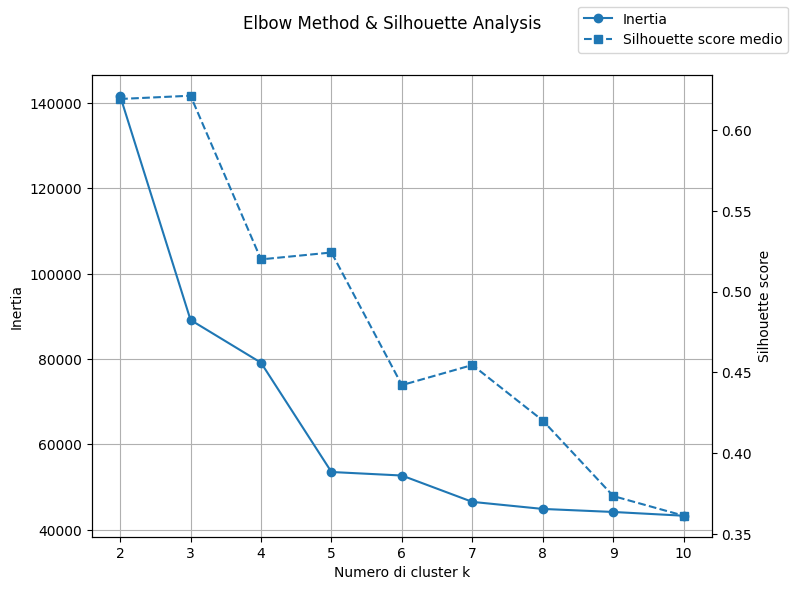
\includegraphics[width=0.7\textwidth]{inertia_elbow.png}
  \caption{Elbow plot: inerzia in funzione di $k$.}
  \label{fig:elbow}
\end{figure}
La riduzione di inerzia da $k=2$ a $k=3$ è significativa, mentre per numeri di cluster maggiori il guadagno in compattezza è minore.

\section{Visualizzazioni 2D}
\subsection{PCA 2D}
La proiezione PCA bidimensionale evidenzia i tre cluster:
\begin{figure}[h!]
  \centering
  % Sostituire con il grafico reale
  \IfFileExists{pca2d.png}{%
    \includegraphics[width=0.7\textwidth]{pca2d.png}%
  }{%
    \fbox{Figura non trovata: pca2d.png}%
  }
  \caption{Distribuzione dei cluster (PCA 2D).}
  \label{fig:pca}
\end{figure}
\begin{itemize}
  \item Cluster 1 (arancione): gruppo molto compatto in alto a sinistra.
  \item Cluster 2 (verde): compatto nella parte bassa con forma a "U".
  \item Cluster 0 (blu): il più numeroso (~60\% dei punti), sparso e a forma di mezzaluna a destra.
\end{itemize}

\begin{figure}[h!]
  \centering
  % Sostituire con il grafico reale
  \IfFileExists{tsne2d.png}{%
    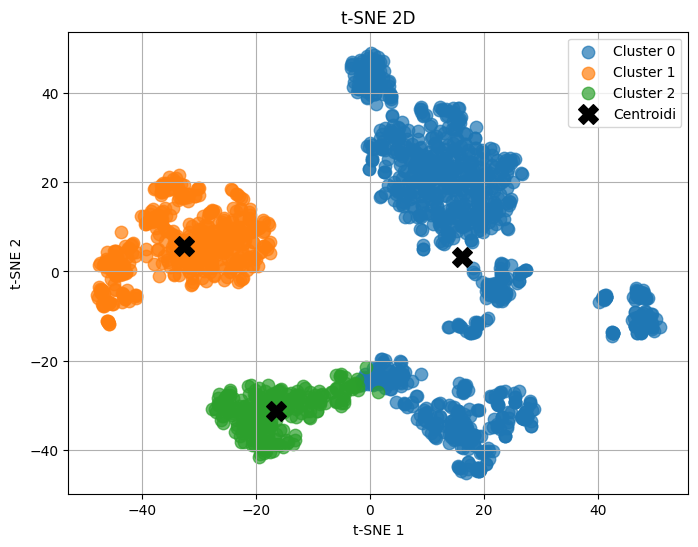
\includegraphics[width=0.7\textwidth]{tsne2d.png}%
  }{%
    \fbox{Figura non trovata: tsne2d.png}%
  }
  \caption{Distribuzione dei cluster (t-SNE 2D).}
  \label{fig:tsne}
\end{figure}

\section{Distribuzione dei Cluster}
La tabella seguente riassume la dimensione e la percentuale di ciascun cluster sul totale dei campioni:
\begin{table}[h!]
  \centering
  \begin{tabular}{lrr}
    \toprule
    Cluster & N. elementi & \% sul totale \\
    \midrule
    0 & 1060 & 59.79\% \\
    1 & 453  & 25.55\% \\
    2 & 260  & 14.66\% \\
    \bottomrule
  \end{tabular}
  \caption{Dimensione e percentuale di ogni cluster.}
  \label{tab:distribution}
\end{table}
Il Cluster 0 è dominante e più eterogeneo; i Cluster 1 e 2 sono più piccoli e densi.

\section{Conclusioni e Proposte}
La scelta di $k=3$ è giustificata dal massimo silhouette score e dall'appiattimento dell'Elbow plot. Tuttavia, il grande Cluster 0 potrebbe contenere sottogruppi di interesse:
\begin{itemize}
  \item Applicare un secondo livello di clustering su Cluster 0 per distinguere sfumature interne.
  \item Valutare altri indici (Davies–Bouldin, Calinski–Harabasz) per una conferma alternativa.
  \item Se l'obiettivo è una netta distinzione tra risposte "lecite" e "jailbreak", considerare $k=2$, con $k=3$ riservato all'analisi di eccezioni.
  \item Validare le assegnazioni su un sottoinsieme etichettato manualmente per misurare precision/recall.
\end{itemize}

\end{document}